\documentclass{beamer}

\title{The Impact of Anthropogenic Forcing on ENSO Amplitude}
\author{Ben Goldman}
\date{\today}

\usepackage{natbib}
\usepackage{tikz}
\usepackage{varwidth}
\usepackage{hyperref}

\usetheme{ben}
\setbeamersize{description width=0.5cm}

\usetikzlibrary{arrows,snakes,backgrounds}
\tikzstyle{process}=[rectangle, draw=process, fill=process!20, line width = 0.3mm]
\tikzstyle{data}=[rectangle, draw=data, fill=data!20, line width = 0.3mm]
\tikzstyle{tight}=[node distance = 0.5in]
\tikzstyle{loose}=[node distance = 2in]
\definecolor{process}{HTML}{3d5f8f}
\definecolor{data}{HTML}{8f6d3d}

\newcommand{\myfig}[3]{
  \begin{figure}
    \centering
    \includegraphics[width=\textwidth]{figures/#1}
    \caption{#2}
    \label{fig:#3}
  \end{figure}
}
\renewcommand{\bibsection}{}

\begin{document}

\maketitle

\begin{frame}{Climate Change: Global Warming vs. Climate Variability}
  \begin{figure}
    \centering
    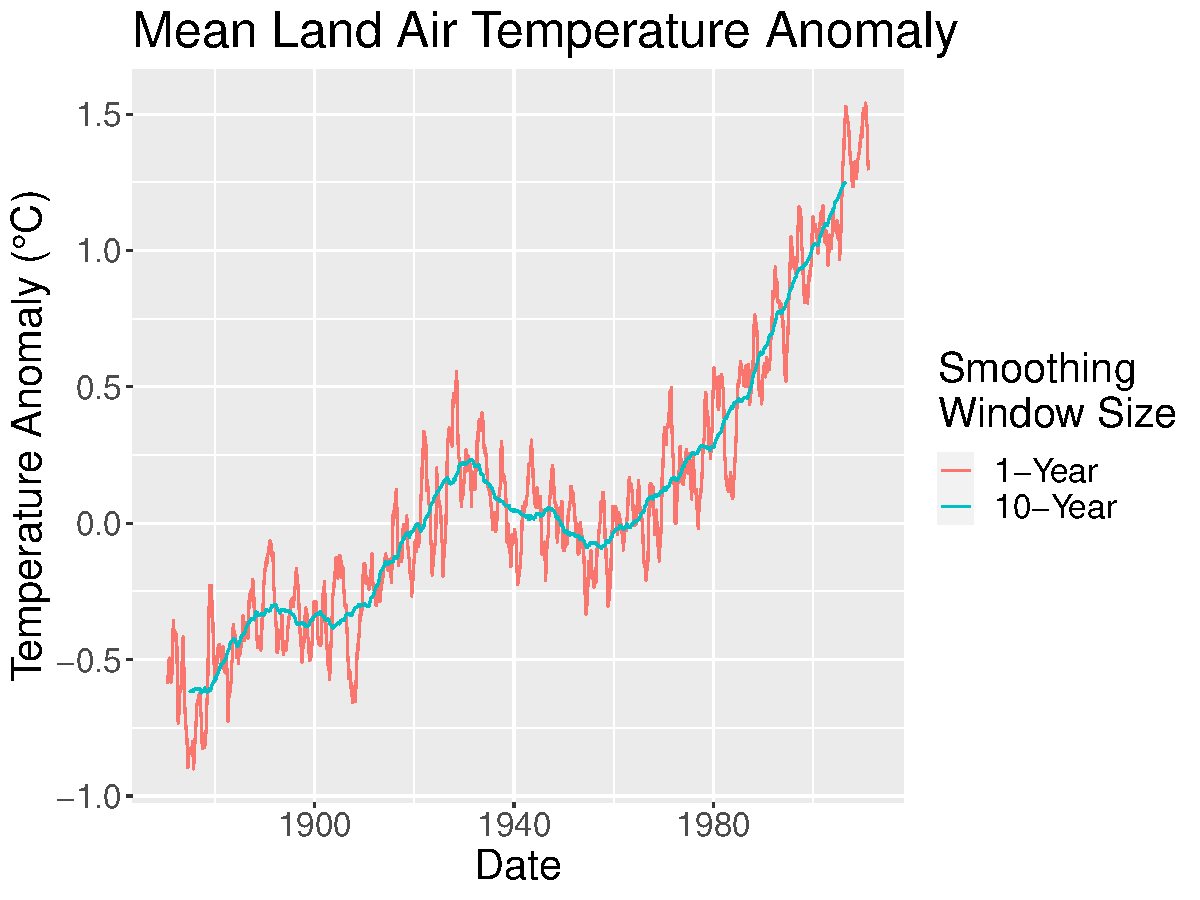
\includegraphics[width=0.8\textwidth]{figures/intro_fig_3.pdf}
    \caption{Global mean land air temperature in GISSTEMP 4 dataset. \citep{gistemp2019giss} and \citep{lenssen2019improvements}}
    \label{fig:woohoo}
  \end{figure}
\end{frame}

\begin{frame}{Greenhouse Gasses and Friends}
  \begin{columns}
    \column{0.5\textwidth}
    \begin{itemize}
    \item \alert{Forcing}: any external factor that affects climate.
      \begin{description}
      \item[\alert{GHG}] Greenhouse gasses
      \item[\alert{AER}] Aerosols (natural: volcanic ash, artificial: smoke)
      \item[\alert{BMB}] Biomass burning
      \item[\alert{LULC}] Land use/cover (deforestation, desertification)
      \end{description}
    \end{itemize}
    \column{0.6\textwidth}
    \myfig{greenhouse_Effect.jpg}{Factors that contribute to the greenhouse effect. \url{https://www.coolaustralia.org/the-greenhouse-effect-secondary}}{this}
  \end{columns}
\end{frame}

\begin{frame}{El Niño, La Niña, and ENSO}
  \begin{figure}
    \begin{columns}
      \column{0.5\textwidth}
      \begin{itemize}
      \item ENSO = El Niño/Southern Oscillation
      \item El Niño is the warm phase, and La Niña is the cool phase.
      \item Warming and cooling of the Pacific Ocean.
      \item Affects human societies through temperature and rainfall. \citep{ropelewski1987global}
      \end{itemize}
      \caption{Comparison of SST anomaly between 1975 La Niña event and 1997 El Niño event in HadISST 1 dataset. \citep{rayner2003global}}
      \column{0.6\textwidth}
      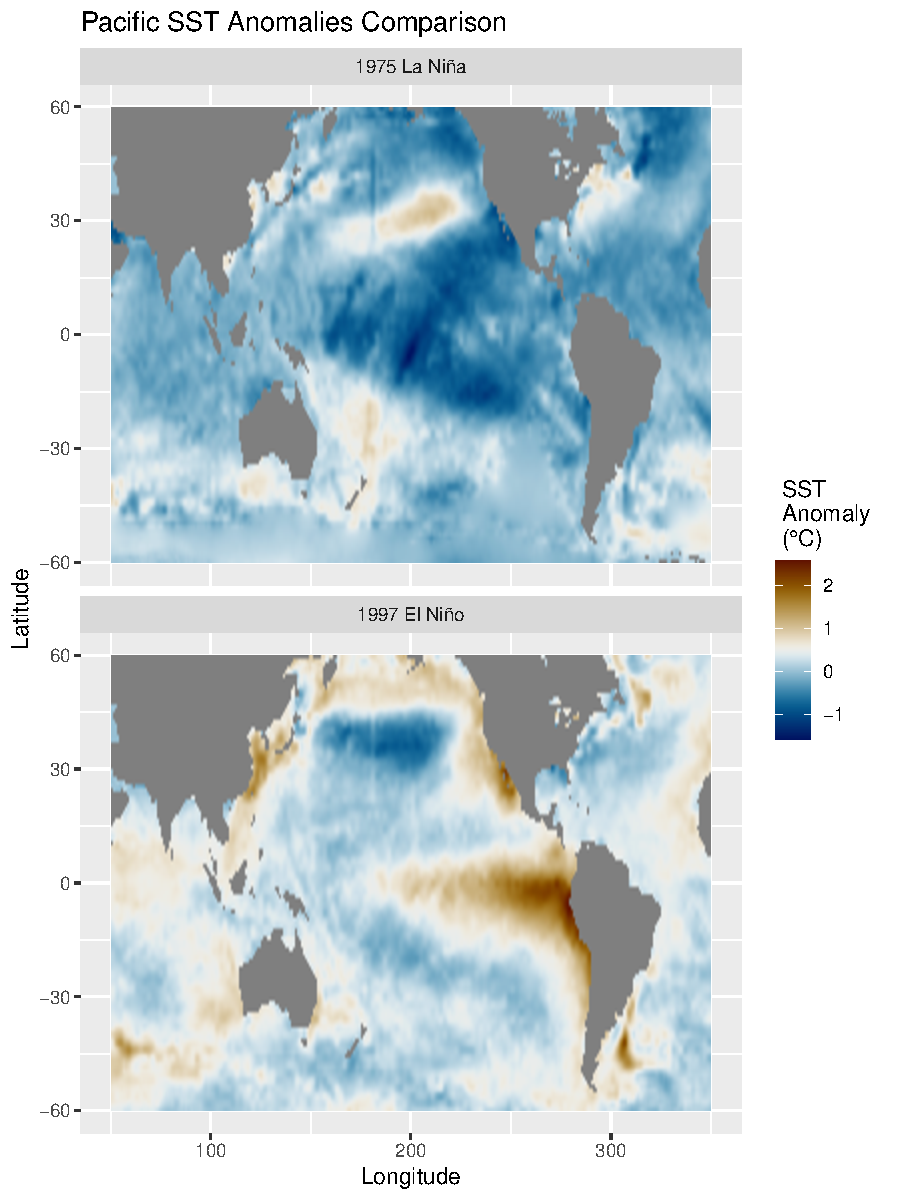
\includegraphics[width = \textwidth]{figures/intro_fig.pdf}
    \end{columns}
  \end{figure}
\end{frame}

\begin{frame}{Review of Literature}
  \begin{itemize}
  \item ENSO's properties observed vary across different decades. \citep{lubbecke2014assessing}.
  \item Weakened ENSO during the Ice Age due to reduced CO$_2$ levels \citep{zhu2017reduced}.
  \item Models show possible increasing ENSO activity in the future \citep{zheng2017response} and \citep{maher2018enso}.
  \end{itemize}
\end{frame}

\begin{frame}{Gap and Questions}
  \alert{Gap}
  \begin{itemize}
  \item Little research using a large ensemble to examine the effect of individual factors on ENSO.
  \item Considerable disagreement between studies on whether ENSO will strengthen or weaken due to global warming
  \end{itemize}
  \alert{Questions}
  \begin{enumerate}
  \item Do the CESM1 and CESM2 predict increased or decreased ENSO intensity in the future?
  \item Is the predicted increase (or decrease) due to human activities?
  \end{enumerate}
\end{frame}

\section{Methods and Results}

\begin{frame}{Data: Community Earth System Model}
  \begin{itemize}
  \item Community Earth System Model (CESM) Versions 1 and 2 \citep{kay2015community} \citep{danabasoglu2020community}.
  \item Predicts climate over 21st century with global warming.
  \item Ensemble: collection of multiple simulations.
  \item Single forcing ensembles that represent influence of single factor.
  \end{itemize}
\end{frame}

\begin{frame}{Measuring ENSO Intensity}
  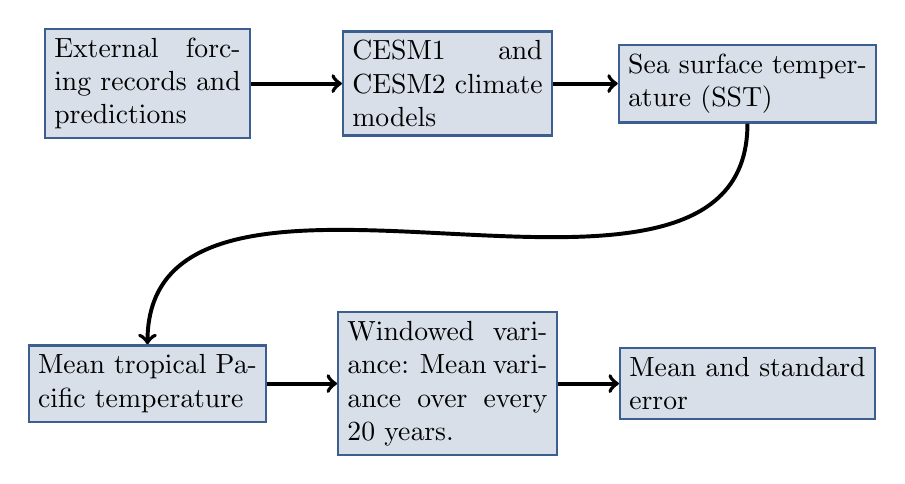
\begin{tikzpicture}[node distance = 1.5in, line width = 0.5mm]
    \node [process] (input) {
      \begin{varwidth}{1.2in}
        External forcing records and predictions
      \end{varwidth}};
    \node [process] (model) [right of=input] {
      \begin{varwidth}{1.2in}
        CESM1 and CESM2 climate models
      \end{varwidth}};
    \node [process] (output) [right of=model] {
      \begin{varwidth}{1.2in}
        Sea surface temperature (SST)
      \end{varwidth}};
    \node [process] (nino) [below of=input] {
      \begin{varwidth}{1.2in}
        Mean tropical Pacific temperature
      \end{varwidth}};
    \node [process] (variance) [right of=nino] {
      \begin{varwidth}{1.0in}
        Windowed variance: Mean variance over every 20 years.
      \end{varwidth}};
    \node [process] (intensity) [right of=variance] {
      \begin{varwidth}{1.2in}
        Mean and standard error
      \end{varwidth}};
    \draw [->] (input) to (model);
    \draw [->] (model) to (output);
    \draw [->] (output) to [out = 270, in = 90] (nino);
    \draw [->] (nino) to (variance);
    \draw [->] (variance) to (intensity);
  \end{tikzpicture}
\end{frame}

\begin{frame}{ENSO is Becoming Stronger}
  \begin{columns}
    \column{0.5\textwidth}
    \begin{itemize}
    \item Increase in ENSO intensity in both ensembles. (Exceeds 2 standard errors)
    \item Increase slows down in CESM1 and decreases in CESM2 after around 2050.
    \end{itemize}
    \column{0.5\textwidth}
    \begin{figure}
      \begin{tikzpicture}
        \node[anchor=south west,inner sep=0] at (0,0) {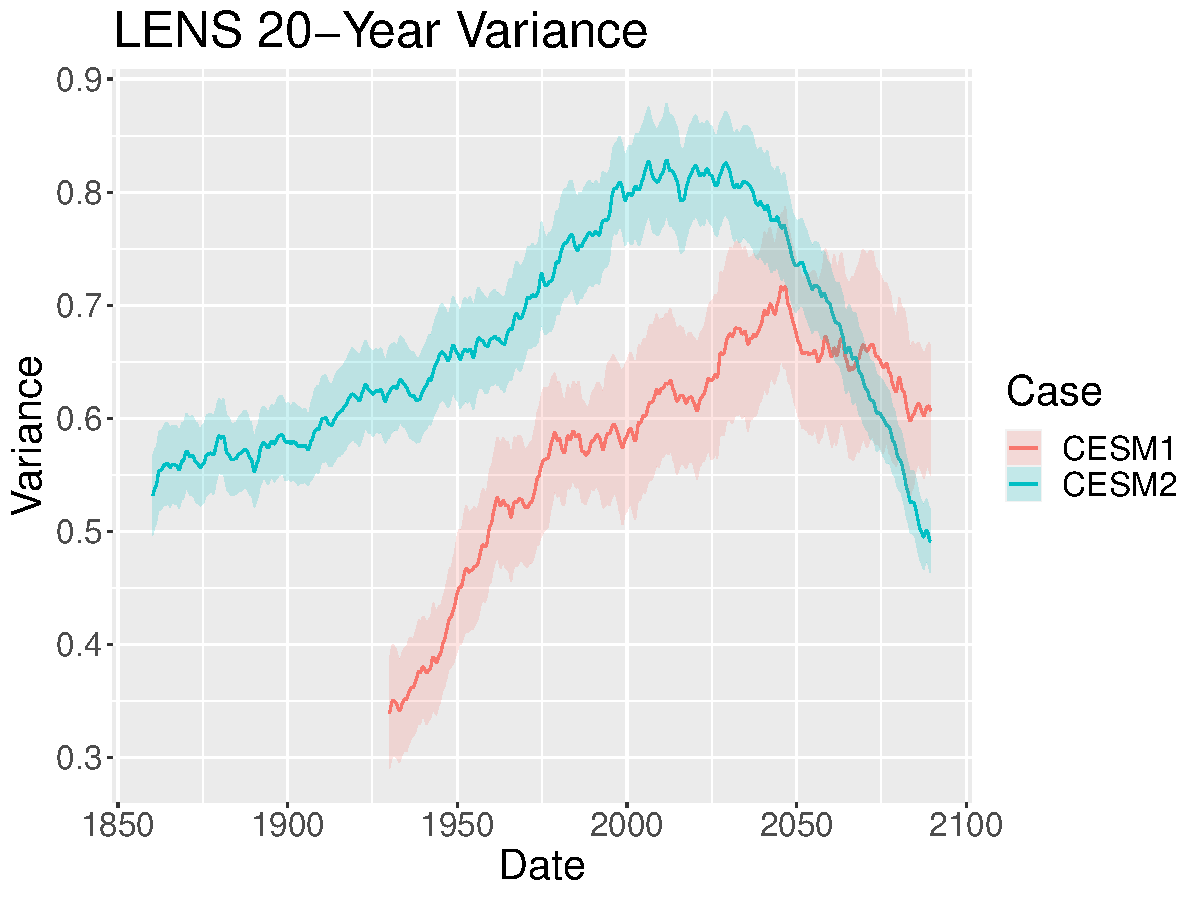
\includegraphics[width=\textwidth]{figures/ff_compare.pdf}};
        \coordinate (a) at (0.5, 1.5);
        \node [red] (b) at (1.0, 1.0) {
          \begin{varwidth}{0.6in}
            Increasing variance
          \end{varwidth}};
        \coordinate (c) at (3.0, 1.5) {};
        \draw[red, |-|] (a) to (c);

        \coordinate (d) at (3.2, 1.5);
        \node [red] (e) at (3.5, 1.0) {
          \begin{varwidth}{0.6in}
            Decreasing variance
          \end{varwidth}};
        \coordinate (f) at (4.3, 1.5) {};
        \draw[red, |-|] (d) to (f);
      \end{tikzpicture}
      \caption{ENSO intensity ensemble mean and standard error for CESM1 and CESM2}
      \label{ff_compare}
    \end{figure}
  \end{columns}
\end{frame}

\begin{frame}{Influence of Aerosols and Greenhouse Gasses}
  \begin{columns}
    \column{0.65\textwidth}
    \begin{itemize}
    \item Influence of each factor on ENSO amplitude.
    \item Increased variance due to greenhouse gas emissions.
    \item Somewhat increased variance from aerosol emissions, but not linear.
    \end{itemize}
    \alert{Takeaway:} Human activities are triggering predicted strengthening of ENSO.
    \column{0.5\textwidth}
    \myfig{cesm1_sf_4.pdf}{Influence of GHG, AER, and BMB forcing on ENSO amplitude in CESM1}{cesm1_sf_4}
  \end{columns}
\end{frame}

% \begin{frame}{Correlation With Ocean Temperature}
%   \begin{columns}
%     \column{0.65\textwidth}
%     \begin{itemize}
%     \item Correlation coefficient between ocean temperature and ENSO amplitude.
%     \item Negative coefficient in subsurface layer.
%     \item Positive coefficient in surface layer.
%     \item Suggests that ocean stratification may be mediating global warming influence on ENSO.
%     \item Difference in heating modifies mechanics of ENSO cycle.
%     \end{itemize}
%     \column{0.5\textwidth}
%     \myfig{tempdt.pdf}{Correlation coefficient between ENSO amplitude and ocean temperature in equatorial cross-section in the fully-forced CESM1 ensemble}{tempdt}
%   \end{columns}
% \end{frame}

\begin{frame}{Wavelet Analysis}
  \begin{columns}
    \column{0.5\textwidth}
    \begin{itemize}
    \item Separate ENSO record into changes in period over time.
    \item In CESM1, increase in ENSO intensity is mainly strengthening of longer-period cycle.
    \item In CESM2, longer-period ENSO weakens after 2025.
    \item Indicates that longer frequency bands are more susceptible to climate change.
    \end{itemize}
    \column{0.5\textwidth}
    \myfig{wavelet3.pdf}{Wavelet power spectrum for the Niño 3.4 index in the fully-forced CESM1 and CESM2 ensembles}{wavelet2}
  \end{columns}
\end{frame}

% SPLIT UP CONCLUSIONS DISCUSSION

\begin{frame}{Discussion}
  \begin{itemize}
  \item Rising greenhouse gas levels strengthen ENSO cycle.
  \item Aerosol influence is nonlinear because aerosol levels are not purely increasing.
  \item Stronger ENSO may lead to greater temperature variability and extreme weather.
  \item External forcing affects lower frequency ENSO more.
  \end{itemize}
\end{frame}

\begin{frame}{Limitations and Applications}
  Limitations:
  \begin{itemize}
  \item Niño 3.4 index shown to be inaccurate for some models \citep{cai2018increased}.
  \item CESM may contain biases.
  \item Models are only an approximation of the Earth's actual climate.
  \end{itemize}
  Application: to improve our ability to predict ENSO and help people prepare for increased likelihood of extreme weather.
\end{frame}

\begin{frame}{Acknowledgments}
  \begin{itemize}
  \item This material is based upon work supported by the National Center for Atmospheric Research, which is a major facility sponsored by the National Science Foundation under Cooperative Agreement No. 1852977.
  \item Thank you to my teacher, my family, and my mentor!
  \item Software used: R, ncdf4, zoo, dplyr, ggplot2, WaveletComp, reshape2, nco.
  \end{itemize}
\end{frame}

\begin{frame}{Role of Mentor and Student}
  \begin{columns}[t]
    \column{.5\textwidth}
    Student:
    \begin{itemize}
    \item Analyze raw data on computer
    \item Produce graphics for analysis and publication
    \item Write documentation
    \item Identify key features of results
    \end{itemize}
    \column{.5\textwidth}
    Mentor:
    \begin{itemize}
    \item Review student writing
    \item Interpret results in the context of climatology
    \item Conduct parallel analysis
    \item Provide raw data from facility
    \end{itemize}
  \end{columns}
\end{frame}

\begin{frame}{References}
  \bibliographystyle{apalike}
  \fontsize{4pt}{5}\selectfont
  \bibliography{references.bib}
\end{frame}

\end{document}





% hi
